%\documentclass{IEEEtran}
\documentclass{IEEEtran}
\IEEEoverridecommandlockouts
% The preceding line is only needed to identify funding in the first footnote. If that is unneeded, please comment it out.
\usepackage{cite}
\usepackage{amsmath,amssymb,amsfonts}
\usepackage{algorithmic}
\usepackage{graphicx}
\usepackage{textcomp}
\usepackage{xcolor}
\def\BibTeX{{\rm B\kern-.05em{\sc i\kern-.025em b}\kern-.08em
    T\kern-.1667em\lower.7ex\hbox{E}\kern-.125emX}}


\begin{document}

\title{Completeness-Security Gap in LSM-based provenance capture mechanisms?\\
{\footnotesize}
\thanks{}
}

\author{\IEEEauthorblockN{ Aarti Kashyap}
\IEEEauthorblockA{\textit{Electrical and Computer Engineering} \\
\textit{ University of British Columbia}\\
Vancouver, Canada \\
kaarti.sr@gmail.com}


}

\maketitle
\large
\begin{abstract}
Information flow control at the Operating system level has been an active area of interest for a long time. Using information flow control techniques we can describe how data came to be in its present form by gathering metadata that describes the history of each object being processed on the system. This is called as data provenance. Data provenance has many uses, from forensics and security to aiding the reproducibility of scientific experiments. The existing implementations for Linux are based on the Linux Security Modules (LSM) framework which implements hooks at specific points to control operations on kernel objects and a set of opaque security fields in kernel data structures for maintaining security attributes. 
However, while past work on verification of LSMs addressed the reliability of information flow control system built on LSMs, no one has addressed the security of information flow control system built on LSMs. In this work, we show that the current LSM interface captures all security-related flows in the kernel. Next, given the provenance captured at these points, we explore if the security violation shows up as an anomaly in the provenance graph. 
\end{abstract}



\begin{IEEEkeywords}
	Data provenance, Whole-system provenance, Linux kernel
\end{IEEEkeywords}


\section{Introduction}
System security is race between the attackers and the defenders. The attackers, adapt their attack model based on the defense mechanisms being deployed on the systems. The designers of the systems can build a completely correct system using formal methods such as theorem proving and model checking \cite{b4}. However, this only proves the correctness properties of the systems such as " Making sure that the system is following the correct protocol " or  " the shared memory allocation is done efficiently". The attacker can make sure that there is no violation in these properties and still manage to attack the system. In order to beat the attacker in this game, several security based mitigation techniques are proposed, which lack complete security coverage. \cite{b5}. Hence, in order to obtain a full or a wider coverage of the system, using provenance-based techniques is an ideal way to proceed. \cite{b6}

Provenance has many different definitions when used in different contexts. The simplest way to define provenance is a formal set of documents, to understand the beginning of something's existence and origin. These documents can be used to guide  authenticity or quality of the item. In a computing context, data provenance represents, in a formal manner, different relationships between entities (data items), activities (data transitions) and agents (which cause the transition). In other words, it can be understood as a formal set of documents which help in understanding the data existence and it's flow to trace its integrity (quality). \cite{b1}

Information flow tracking is a security mechanism designed to monitor how sensitive information spreads in a system. In data provenance context, information flow tracking is used to track the data and is be further used to put limits on the dissemination of a piece of sensitive data once it's out of it's container of information. This allows high level policies such as " my banking information will not be sent outside my system " or " my banking information will not be mixed with my wife's banking information" to be enforced easily.  \cite{b2}. An explicit information flow is defined as the copy, usually partial, of the content of one container of information to another. \cite{b3}

Data provenance with a completeness property ensures that all the information flows of the data within the system are being recorded. Pasquier et. al \cite{b6} in his work on Run-time Analysis of Whole-system provenance ensures the completeness and accuracy of the provenance capture mechanism. They further use Georget et al. \cite{b3} formalism to show that all the information flows between the kernel objects are properly recorded. However, this does not prove that all the security related flows are also being captured by the system. 


\begin{figure}
	\centering
	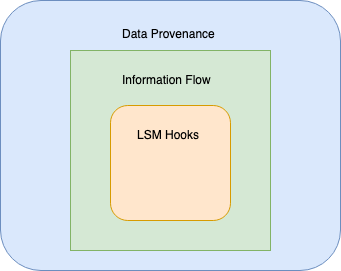
\includegraphics[width=0.7\linewidth]{Architecture-diagram}
	\caption[]{High-level Architectural view. A structured way to formalize whole-system data provenance is to formalize if all the information flows are being captured. In order to make sure that all information flows are being captured we need to make use of LSM to insert hooks at every point in the kernel where a user-level system call is about to result in access to an important internal kernel object.}
	\label{fig:architecture-diagram}
\end{figure}

\begin{figure}
	\centering
	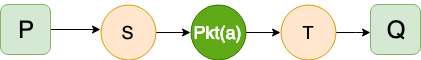
\includegraphics[width=0.7\linewidth]{DAG}
	\caption{A simple provenance DAG: a process P sends packet Pkt(a) to process Q using the sockets S and T.}
	\label{fig:dag}
\end{figure}





Hence, as a part of this work we try to answer the question about complete and security related flows of the system using a whole-system provenance capture called Camflow.\cite{b7}

The first part of the challenge includes answering the question if the completeness formalism is enough to detect all security related flows. Xueyuan et al. uses whole-system provenance capture tool for fault-detection \cite{b8}. Pasquier et. al. \cite{b6} shows that it's possible to detect intrusions during run-time of the system. However, is it enough to detect all sorts of data leaks and/or intrusions is one question we try to answer as a part of this work. This analysis has been performed for Linux Kernel 4.3. We try to see if the formalism still holds for the updated version.     


The second contribution of our work is, if indeed Camflow \cite{b7}  is able to capture all security-related flows, do they all show up as an anomaly in the provenance-graph. The provenance-graph is constructed from the data captured from all the security-related flows in the system. 


\section{Background}
We conduct an analysis to see if the current version of the information flow patch applied to CamFlow is capable enought to catch all security violations. In order to do so, we make use of three open-source tools/libraries/patches CamFlow, GraphChi and complete flow capture formalism proposed by inria. 

\subsection{CamFlow} 

As we have discussed before data provenance records the chronology of  ownership, change and movement of an object or a resource. There are many provenance capture systems available including PASS \cite{b10}, Hi-Fi\cite{b11}, Linux Provenance Module \cite{b12} and CamFlow\cite{b9}. The capture mechanism is built on the Linux Security Modules (LSM). LSM is a framework that allows the kernel to support variety of computer security models while avoiding favoritism towards any of the security implementations. 

We chose CamFlow for testing our hypothesis because it adopts the LSM architecture and support for NetFilters which makes it a maintainable practical whole-system provenance implementation .CamFlow maintains a patch based on Georget et al's \cite{b3}formalism which provides completeness guarantees. The fact that Cam-flow provides completeness guarantees, its a strong choice for researchers to use it as a fault-detection tool \cite{b8}. Pasquier et al. uses CamFlow to perform a run-time analysis of whole-system provenance to find intrusions \cite{b6}. However, since the completeness guarantees are specific to kernel version 4.3, we want to provide a formalism which shows that it holds for the updated kernel versions. 

\subsection{GraphChi}

The representation of the provenance data is in form of a directed acyclic graph (DAG). Every node in the DAG represents an entity, an activity or an agent. Each directed edge represents interaction between each node. Fig.2 represents a simple example. In our context, entities are kernel objects, activities are tasks; and agents are users and groups. 

We use GraphChi, a vertex-centric graph processing model to generate program models and to generate anomalies. The purpose of utilizing GraphChi is to answer that in case of security violations in the system, are the anomalies reflected in the graphs. 


\subsection{title}
\subsection{Equations}
Number equations consecutively. To make your 
equations more compact, you may use the solidus (~/~), the exp function, or 
appropriate exponents. Italicize Roman symbols for quantities and variables, 
but not Greek symbols. Use a long dash rather than a hyphen for a minus 
sign. Punctuate equations with commas or periods when they are part of a 
sentence, as in:
\begin{equation}
a+b=\gamma\label{eq}
\end{equation}

Be sure that the 
symbols in your equation have been defined before or immediately following 
the equation. Use ``\eqref{eq}'', not ``Eq.~\eqref{eq}'' or ``equation \eqref{eq}'', except at 
the beginning of a sentence: ``Equation \eqref{eq} is . . .''







\subsection{Figures and Tables}
\paragraph{Positioning Figures and Tables} Place figures and tables at the top and 
bottom of columns. Avoid placing them in the middle of columns. Large 
figures and tables may span across both columns. Figure captions should be 
below the figures; table heads should appear above the tables. Insert 
figures and tables after they are cited in the text. Use the abbreviation 
``Fig.~\ref{fig}'', even at the beginning of a sentence.

\begin{table}[htbp]
\caption{Table Type Styles}
\begin{center}
\begin{tabular}{|c|c|c|c|}
\hline
\textbf{Table}&\multicolumn{3}{|c|}{\textbf{Table Column Head}} \\
\cline{2-4} 
\textbf{Head} & \textbf{\textit{Table column subhead}}& \textbf{\textit{Subhead}}& \textbf{\textit{Subhead}} \\
\hline
copy& More table copy$^{\mathrm{a}}$& &  \\
\hline
\multicolumn{4}{l}{$^{\mathrm{a}}$Sample of a Table footnote.}
\end{tabular}
\label{tab1}
\end{center}
\end{table}



Figure Labels: Use 8 point Times New Roman for Figure labels. Use words 
rather than symbols or abbreviations when writing Figure axis labels to 
avoid confusing the reader. As an example, write the quantity 
``Magnetization'', or ``Magnetization, M'', not just ``M''. If including 
units in the label, present them within parentheses. Do not label axes only 
with units. In the example, write ``Magnetization (A/m)'' or ``Magnetization 
\{A[m(1)]\}'', not just ``A/m''. Do not label axes with a ratio of 
quantities and units. For example, write ``Temperature (K)'', not 
``Temperature/K''.
\section* {Discussion Topics}
From observations we can 
\section*{Acknowledgment}

This work was done as a part of our term project for CPSC 508. CPSC 508 is a graduate level operating systems course taken by Dr. Margo Seltzer.

\begin{thebibliography}{00}
\bibitem{b1} Lucian Carata, Sherif Akoush, Nikilesh Balakrishnan, Thomas Bytheway,
Ripduman Sohan, Margo Seltzer, Andy Hopper, an ``A Primer on Provenance,'' acmqueue, 2014.
\bibitem{b2} Daniel Crawl and Ilkay Altintas , A Provenance-Based Fault Tolerance Mechanism for
Scientific Workflows.

\bibitem{b3} Laurent Georget, Mathieu Jaume, Guillaume Piolle, ``Verifying the reliability of operating system-level information flow control systems in linux,'' Proceedings of the 5th International FME Workshop on Formal Methods in Software Engineering, FormaliSE ’17, pages 10–16, Piscataway, NJ, USA, 2017. IEEE Press.

\bibitem{b4}GERWIN KLEIN, ``Operating system verification—An overview,"Sadhan ¯ a¯ Vol. 34, Part 1, February 2009, pp. 27–69. © Printed in India

\bibitem{b5} Jonathan Pincus and Brandon Baker , ``Mitigations for Low-Level Coding Vulnerabilities:
Incomparability and Limitations ,'' 2004.


\bibitem{b6}Thomas Pasquier, Xueyuan Han, Thomas Moyer, Adam Bates, Olivier Hermant, David Eyers, Jean Bacon, Margo Seltzer, ``Runtime Analysis of Whole-System Provenance
,''16 pages, 12 figures, 25th ACM Conference on Computer and Communications Security 2018.



\bibitem{b7} Thomas Pasquier, Xueyuan Han, Mark Goldstein, Thomas Moyer, David Eyers, Margo Seltzer, Jean Bacon, Practical Whole-System Provenance Capture
, SoCC '17 Proceedings of the 2017 Symposium on Cloud Computing.


\bibitem{b8} Xueyuan Han, Thomas Pasquier, Tanvi Ranjan, Mark Goldstein, and Margo Seltzer, Harvard University

 , ``FRAPpuccino: Fault-detection through Runtime Analysis of Provenance ,'' HotCloud'17.



\bibitem{b9} PASQUIER, T. F.-M., SINGH, J., BACON, J., AND EYERS, D. , ``Information flow audit for paas clouds.
Cloud Engineering
(IC2E), 2016 IEEE International Conference on (2016), IEEE,
pp. 42–51.


\bibitem{b10} MUNISWAMY-REDDY, K.-K., HOLLAND, D. A., BRAUN, U.,
AND SELTZER, M. I. , `` Provenance-aware storage systems. ,'' In
USENIX Annual Technical Conference, General Track (2006),
pp. 43–56..


\bibitem{b11} POHLY, D. J., MCLAUGHLIN, S., MCDANIEL, P., AND BUTLER, K , ``Hi-fi: collecting high-fidelity whole-system provenance ,'' In Proceedings of the 28th Annual Computer Security Applications Conference (2012), ACM, pp. 259–268.


\bibitem{b12} Adam Bates, Dave (Jing) Tian, and Kevin R.B. Butler , ``Trustworthy Whole-System Provenance
for the Linux Kernel.
24th USENIX Security Symposium, 2015.








\bibitem{b13} PASQUIER, T. F.-M., SINGH, J., BACON, J., AND EYERS, D. , ``Information flow audit for paas clouds.
Cloud Engineering
(IC2E), 2016 IEEE International Conference on (2016), IEEE,
pp. 42–51.


\bibitem{b14} PASQUIER, T. F.-M., SINGH, J., BACON, J., AND EYERS, D. , ``Information flow audit for paas clouds.
Cloud Engineering
(IC2E), 2016 IEEE International Conference on (2016), IEEE,
pp. 42–51.
\end{thebibliography}


\end{document}
